\documentclass[12pt,a4paper]{article}
\usepackage{cmap} % Makes the PDF copiable. See http://tex.stackexchange.com/a/64198/25761
\usepackage[T1]{fontenc}
\usepackage[brazil]{babel}
\usepackage[utf8]{inputenc}
\usepackage{amsmath}
\usepackage{amsfonts}
\usepackage{amssymb}
\usepackage{amsthm}
\usepackage{textcomp} % \degree
\usepackage{gensymb} % \degree
\usepackage[usenames,svgnames,dvipsnames]{xcolor}
\usepackage{hyperref}
\usepackage{multicol}
\usepackage{graphicx}
\usepackage[margin=2cm]{geometry}

\hypersetup{
    colorlinks = true,
    allcolors = {blue}
}

\newcommand*\tg{\operatorname{tg}}
\newcommand*\R{\mathbb{R}}

\newcommand*\tipo{PROVA III}
\newcommand*\turma{NEX152-D}
\newcommand*\disciplina{CDI0001}
\newcommand*\eu{Helder G. G. de Lima}
\newcommand*\data{18/11/2015}

\author{\eu}
\title{\tipo - \disciplina}
\date{\data}

\begin{document}
\thispagestyle{empty}
\newgeometry{margin=2cm,bottom=0.5cm}
\begin{center}

\includegraphics[width=9.0cm]{marca}
\noindent\begin{tabular}{l c c r}
  \textbf{\disciplina (\turma)}
& \textbf{\tipo}
& \textbf{\data}
\end{tabular}
\\ Prof. \eu\footnote{
Este é um material de acesso livre distribuído sob os termos da licença \href{https://creativecommons.org/licenses/by-sa/4.0/deed.pt_BR}{Creative Commons BY-SA 4.0}.}
\end{center}

\noindent Nome do(a) aluno(a): \rule{13cm}{0.01cm}

%\section*{Instruções}
\begin{center}\fbox{
\begin{minipage}{14cm}

{\footnotesize
\begin{itemize}
\renewcommand{\theenumi}{\Roman{enumi}}
\item Identifique-se em todas as folhas.
\item Mantenha o celular e os demais equipamentos eletrônicos desligados durante a prova.
\item Justifique cada resposta com cálculos ou argumentos baseados na teoria estudada.
\item Resolva (integralmente) apenas os itens de que precisar para somar 10,0 pontos.
%\item Escolha \textsc{\textbf{uma}} das 6 questões para \textsc{\textbf{não}} fazer (ela não será corrigida): \framebox(30,10){}

\end{itemize}
}

\end{minipage}
}
\end{center}


%\section*{Questões}

\begin{enumerate}

\item (2,0) Calcule os seguintes limites, utilizando as regras de L'Hôpital quando for apropriado.
\begin{multicols}{2}
\begin{enumerate}
\item $\displaystyle\lim_{x\to\infty} \frac{e^x + 100}{x^2 - 200}$
\item $\displaystyle\lim_{x\to 0} \frac{x-\tg(x)}{x^3}$
\end{enumerate}
\end{multicols}

\item (1,0) Determine os valores de $a$ e $b$ para que $\lim_{x\to0} \dfrac{\sqrt{ax+b}-\sqrt{5}}{x} = \sqrt{5}$.

\item (1,0) Seja $f: [a, b] \to \R$ uma função e $c \in [a, b]$. Explique detalhadamente um procedimento que permita concluir que o maior valor assumido por $f(x)$ ocorre quando $x = c$. Dê um exemplo simples que utilize o procedimento descrito.

\item (3,0) Esboçar $f(x) = \frac{3}{5}x^5 - 4x^3$, explicitando o domínio, simetrias, zeros, intervalos de crescimento e decrescimento, pontos de máximo e mínimo, concavidade, pontos de inflexão, assíntotas e limites que forem relevantes. Não esqueça de justificar suas afirmações!

\item (2,0) Aplique o que se sabe sobre derivadas para calcular as dimensões do retângulo de maior área que pode ser inscrito em uma circunferência de raio 1.
%\includegraphics[width=5.0cm]{retangulo-inscrito.pdf}

\item (1,5) Determine as equações de todas as assíntotas (horizontais, verticais e/ou oblíquas) da função $f(x) = \frac{(x-3)(x+1)}{x-4}$.

\item (1,5) Faça um esboço do gráfico de $f$, assumindo que$f: \R \to \R$ seja uma função derivável cujo gráfico passa por $A=(0, 1)$, e cuja derivada tem o seguinte gráfico:
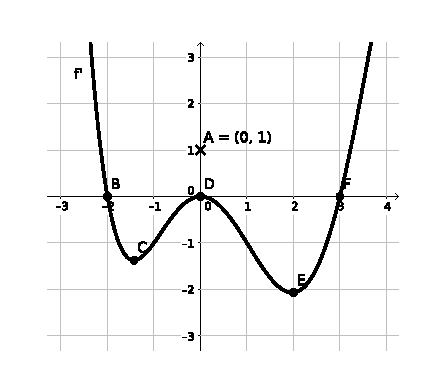
\includegraphics[width=9.0cm]{img/prova-3-nex-grafico-f'}

\end{enumerate}

%\newpage
%\restoregeometry
%\section*{Respostas e observações}
\end{document}
